\documentclass[]{IEEEtran}

\title{Modellazione con SystemC di un sistema hardware per il controllo del livello d'acqua in una cisterna}
\author{Elia Brentarolli - VR433534}

\usepackage{graphicx}
\usepackage[english,italian]{babel}
\usepackage[utf8]{inputenc}
\usepackage{caption}
\usepackage{amsmath}
\begin{document}
\maketitle

\begin{abstract}
	
Questo documento contiene una relazione sul progetto di un modulo HW/SW per il controllo del livello dell'acqua all'interno di una cisterna. Per realizzare ciò si è deciso di applicare un approccio modulare sviluppando dei moduli prima astratti  e, raffinandoli, concreti in seguito sfruttando al meglio la tecnologia offerta da SystemC.

\end{abstract}


\section{Introduzione}
Il progetto svolto prevede l'implementazione di un sistema per stabilizzare in un dato intervallo il livello dell'acqua all'interno di una cisterna tramite un controllore per regolare l'apertura di una valvola ad esso collegata. Per fare ciò il controllore legge il valore del livello e invia alla valvola un comando tra IDLE (valore dentro l'intervallo), OPEN (valore sotto l'intervallo) o CLOSE (valore sopra l'intervallo). Inoltre il controllore invia anche un'apertura massima oltre la quale la valvola non deve aprirsi. In aggiunta a ciò, poiché il controllore invia dati cifrati tramite l'algoritmo  Xtea è necessario un modulo intermedio per le decriptazione di tali dati (figura \ref{scheme}).
\begin{figure*}[ht]
	\centering
	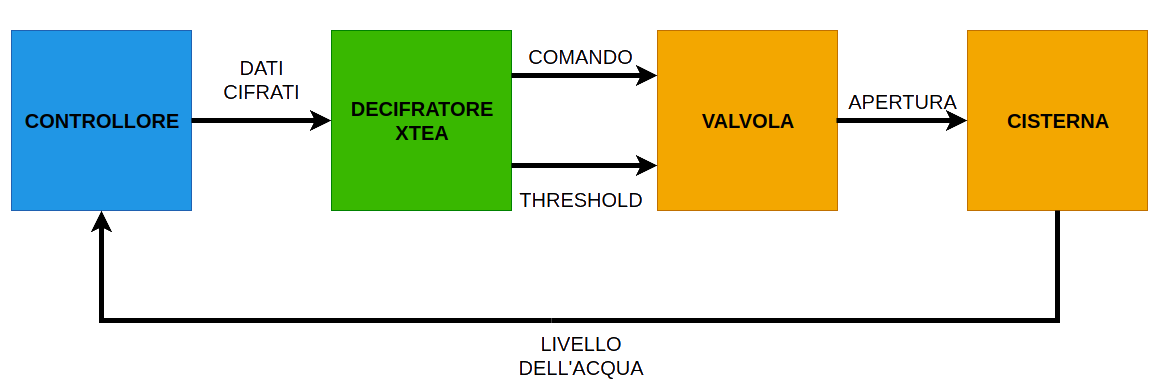
\includegraphics[width=\textwidth]{Images/scheme.png}
	\caption{Schema generale dell'impianto: La cisterna invia dati al controllore che, sulla base di questi, invia dei comandi cifrati prima ad un modulo di decifrazione (Xtea) e poi alla valvola.}
	\label{scheme}
\end{figure*}

Per implementare ciò ci si è basati su un'approccio modulare con riuso di software, partendo da moduli singoli e astratti che sono stati raffinati molteplici volte fino ad arrivare ad un livello implementativo soddisfacente e al contempo che offrisse tutte le funzionalità richieste. Successivamente i moduli sono stati collegati tra loro, sempre con test intermedi, fino ad ottenere un impianto che fornisse risultati buoni nei limiti delle specifiche date.

Per realizzare ciò si sono sfruttate ampiamente  le librerie di SystemC e SystemC-ams in quanto fornite di una molteplice varietà di costrutti utili allo sviluppo e alla simulazione di hardware digitale e di sistemi analogici a tempo continuo. Il progetto realizzato cerca infatti anche di sfruttare al meglio le caratteristiche di SystemC andando ad implementare ogni modulo in uno stile di progettazione o in un livello di astrazione diverso.
\iffalse
Nell'introduzione viene descritto in maniera astratta quello che poi viene dettagliato nel seguito del report. Una buona scaletta per l'introduzione pu\`o essere la seguente:
\begin{itemize}
\item Descrizione ad alto livello delle principali caratteristiche del sistema che si vuole modellare.
\item Descrizione delle motivazioni principali per l'utilizzo delle tecnologie descritte nel corso. Qual'\`e il problema che si vuole risolvere?
\item Descrizione dei passi utilizzati per arrivare all'implementazione finale. Descrivere la motivazione di ciascun passo. La descrizione dei passi dovrebbe formare la descrizione del flusso di lavoro svolto per completare l'assignment.
\item Rapidissima descrizione dei risultati principali.
\end{itemize}

L'introduzione non dovrebbe andare oltre la met\`a della seconda colonna (nel caso a due colonne), o la prima pagina (nel caso a colonna singola): bisogna cercare di essere concisi (e chiari). Alla fine, l'introduzione \`e solo ``chiacchiere'': deve semplicemente rendere chiari quali sono gli obiettivi del lavoro (\emph{e nel caso del corso, deve far capire a me che avete gli obiettivi chiari in testa}). Consiglio: l'introduzione (e spesso l'abstract) \`e l'ultima parte che viene completata.
\fi
\section{Background}

Per la realizzazione del progetto sono stati usati i concetti e le tecnologie riportate in seguito:
\begin{itemize}
	\item SystemC \cite{SystemC}: Libreria standard di classi C++ per la progettazione di sistemi HW o per sistemi ibridi hardware/software a diversi livelli di astrazione.
	\item RTL: Stile di progettazione dell'hardware basato sull'interazione tra le componenti a livello di registri, tramite quindi variazioni sul valore di segnali.
	\item TLM \cite{TLM}: Stile di progettazione più astratto di RTL che si incentra maggiormente sul dialogo che i moduli hanno, piuttosto che sulla loro effettiva funzionalità.
	\item SystemC-AMS \cite{AMS}: Libreria standard di classi C++ basata su systemC per la progettazione di sistemi con funzionalità \emph{analog/mixed-signals}.
	

\end{itemize}

\section{Metodologia applicata}
Come già affermato in precedenza, lo scopo del progetto è quello di realizzare un modulo hardware per la gestione di un impianto per la regolazione del livello dell'acqua all'interno di una cisterna secondo lo schema riportato in figura \ref{scheme}.


Seguendo l'approccio modulare, si è iniziato a sviluppare singolarmente le componenti, partendo dal modulo di criptazione e decriptazione sfruttante l'algoritmo Xtea.
\subsection{XTEA TLM}

Il primo passo fatto nella realizzazione del modulo Xtea è stato quello di dare una sua rappresentazione in TLM e, più specificatamente, nelle tre varianti ovvero TLM UT, TLM LT e TLM AT4. Tuttavia, al contrario del modulo finale che permette solo la decifrazione, si è deciso di andare ad implementare un modulo Xtea completo ovvero che permetta sia criptazione che decriptazione

Partendo con una rappresentazione in TLM UT si è reso subito chiaro che il payload standard usato in TLM non era sufficiente e che andava definita una nuova struttura da agganciare al payload che trasportasse tutte le informazioni utili:
\begin{itemize}
	\item Prima parola da cifrare/decifrare.
	\item Seconda parola da cifrare/decifrare.
	\item Prima chiave.
	\item Seconda chiave.
	\item Terza chiave.
	\item Quarta chiave.
\end{itemize}
Inoltre per non complicare inutilmente la restituzione dei risultati da parte del modulo si è deciso di inserire anche quest'ultimi nella struttura sopra citata:
\begin{itemize}
	\item Primo risultato (corrispondente al calcolo sulla prima parola)
	\item Secondo risultato (corrispondente al calcolo sulla seconda parola)
\end{itemize}
La gestione della scelta tra criptazione e decriptazione è stata fatta usando gli attributi read/write del payload, associando all'opzione ``read'' la funzione di decriptazione e all'opzione ``write'' la funzione di criptazione.
In aggiunta a quanto detto ci si è inoltre resi conto che per implementare tutto l'algoritmo non erano necessari sottomoduli ma un solo ed unico modulo in grado di svolgere entrambe le funzioni. Tale modulo è stato testato collegandolo ad un testbench in grado di fornire degli stimoli adatti e al contempo poter verificare la correttezza dei risultati (figura \ref{scheme2}). Tutto questo è ottenuto tramite l'interfaccia bloccante del TLM offerta da systemC. In particolare in questo caso è stato sufficiente andare ad implementare la funzione \emph{b\_transport}, chiamata dall'initiator (il testbench) e tramite la quale il target (il modulo vero e proprio) viene attivato. Una volta chiamata la funzione l'initiator si mette in attesa fino a quando il target non ha portato a termine la sua funzionalità. Terminato ciò l'initiator può verificare il risultato della computazione andando ad analizzare gli appositi campi presenti nella struttura sopra riportata.
\begin{center}
	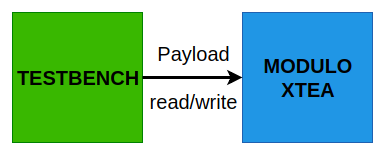
\includegraphics[width=\columnwidth]{Images/scheme2.png}
	\captionof{figure}{Schema riassuntivo dei moduli in TLM UT e TLM LT.}
	\label{scheme2}
\end{center}
Si vuole infine far notare che, poiché l'approccio TLM si incentra fortemente sulla comunicazione tra i moduli piuttosto che sulla loro effettiva funzionalità, si è deciso di implementare l'algoritmo Xtea come due funzioni C++ definite all'interno del modulo e chiamate all'occorrenza.

Successivamente si è raffinato il modulo passando ad una rappresentazione in TLM LT. Il passaggio non è stato per nulla complicato poiché non è stato necessario andare a toccare nè la struttura del payload nè le funzionalità del modulo in sè. Ciò che è stato fatto è stato di aggiungere una nozione di tempo all'interno del sistema, tramite delle attese nel modulo atte a simulare il tempo speso nella computazione e inserendo all'interno del testbench il concetto di temporal decoupling. 

Infine si è passati ad una rappresentazione a livello TLM AT4. Sebbene anche in questo caso non sia stato necessario andare a toccare in modo pesante le funzionalità del modulo in sè, l'implementazione del protocollo TLM AT4 (che prevede una comunicazione bidirezionale tra initiator e target a differenza dei protocolli precedenti) all'interno del testbench ne ha cambiato in modo significativo la struttura in quanto necessario avere un'interfaccia con la quale il modulo Xtea potesse comunicare (figura \ref{scheme3}). In questo caso quindi si è dovuto andare ad implementare due interfacce, una per l'initiator ed una per il target in modo che i due moduli possano dialogare tra loro senza bloccarsi a dover attendere una risposta. Uno schema più accurato può essere osservato nella figura \ref{scheme4}. Terminata anche la rappresentazione in TLM AT4 si è poi passato ad analizzare quanto le rappresentazioni precedenti avevano fornito per poter ricavare delle informazioni utili alla rappresentazione successiva, ovvero ad RT. Essendo di per sè il modulo da implementare non troppo complesso il lavoro fatto a questo livello di astrazione non ha fornito troppe informazioni utili per una futura suddivisione in sottomoduli ma ha fornito un essenziale aiuto per andare a definire le possibili porte di ingresso e uscita che questa componente deve avere partendo dalla struttura del payload che era stata necessaria definire. Inoltre la rappresentazione in AT4 ha messo in evidenza la necessità di due ulteriori porte da aggiungere al modulo tramite le quali il testbench possa avviare il modulo alla computazione e con le quali il modulo possa comunicare la fine della computazione.
\begin{center}
	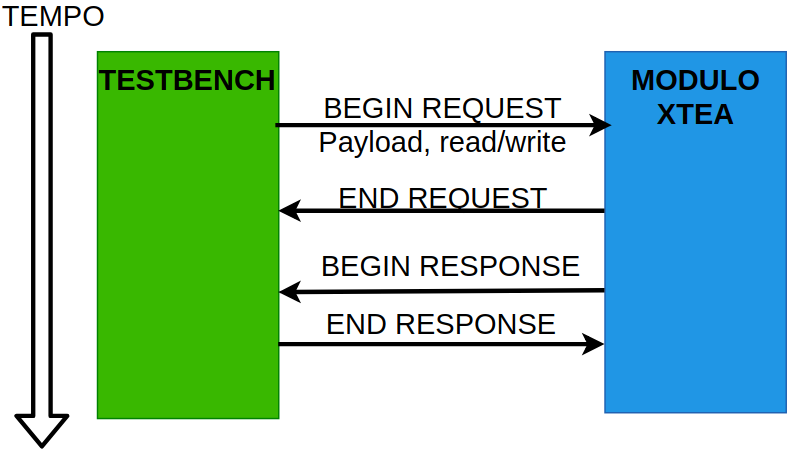
\includegraphics[width=\columnwidth]{Images/scheme3.png}
	\captionof{figure}{Schema riassuntivo dei moduli in TLM AT4.}
	\label{scheme3}
\end{center}
\begin{figure*}[ht]
	\centering
	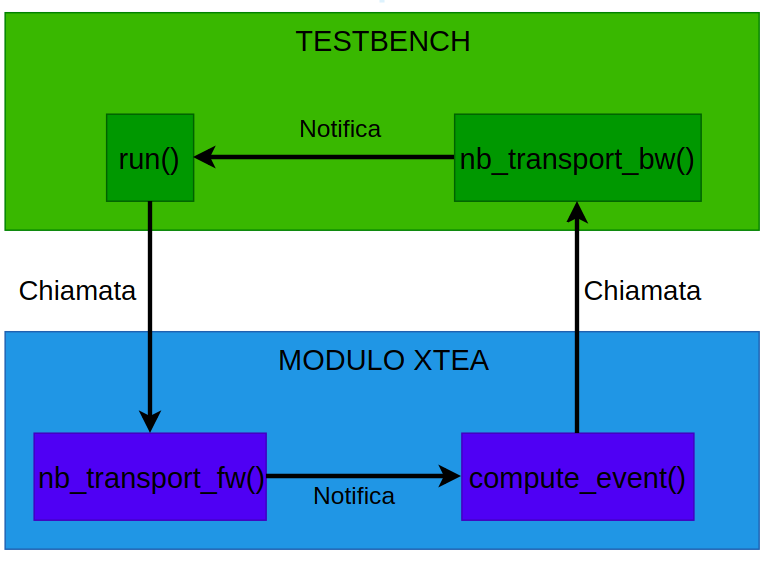
\includegraphics[width=\columnwidth]{Images/scheme4.png}
	\caption{Schema del comportamento dei moduli nella loro rappresentazione in TLM AT4. Il testbench, ad un certo punto del metodo run, chiama la funzione nb\_transport\_fw del target e si mette in di un evento che solo nb\_transport\_bw può generare. A questo punto il metodo nb\_transport\_fw del target attiva un evento che sblocca la funzione compute\_event precedentemente messa in attesa. Al termine di questa viene chiamato il metodo nb\_transport\_bw che riattiva il metodo run.}
	\label{scheme4}
\end{figure*}
\subsection{XTEA RTL}
Successivamente alla rappresentazione in TLM si è passati a quella RTL. Come detto in precedenza alla fine dell'analisi fornita dal TLM si era ottenuta una rappresentazione abbastanza accurata dell'interfaccia che il modulo doveva avere a partire dai campi del payload e dalla necessità di dialogo con il testbench. È stata quindi eseguita la seguente mappatura:
\begin{itemize}
	\item Campi della struttura usati nella funzione $\rightarrow$ Porte di input.
	\item Campi della struttura usati per salvare i risultati della funzione $\rightarrow$ Porte di output.
	\item Attributo read/write del payload $\rightarrow$ Porta di input per la modalità.
	\item Funzione per avviare la computazione $\rightarrow$ Porta di input ``din''.
	\item Funzione per il ritorno  della computazione  $\rightarrow$ Porta di output ``dout''.
\end{itemize}
Oltre a ciò sono state inserite due ulteriori porte di input, ovvero quella dedicata al clock ed al reset in quanto la progettazione ad RT prevede la realizzazione di moduli sincroni. La figura \ref{scheme5} mostra il risultato del passaggio da TLM a RTL. 

\begin{center}
	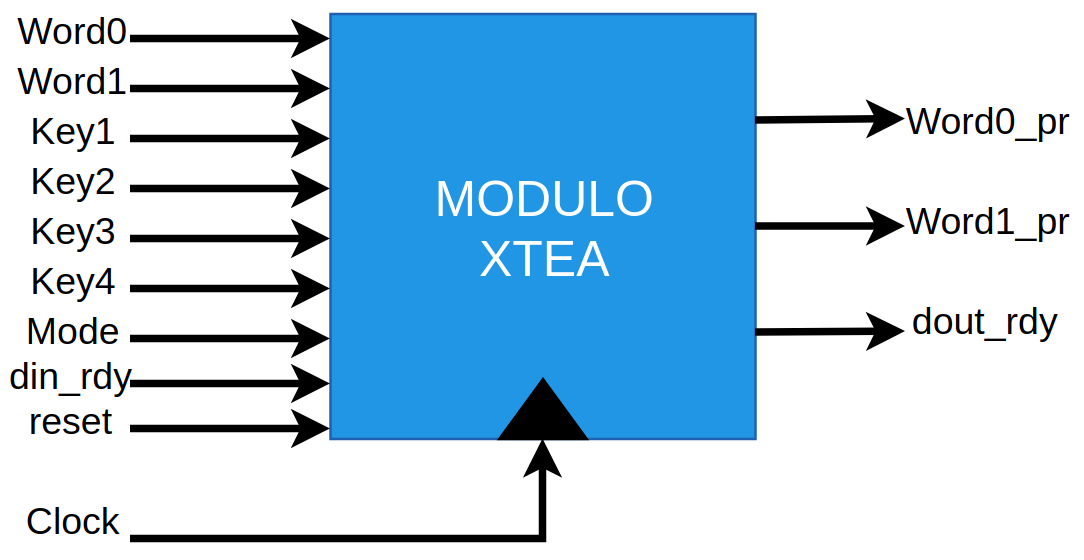
\includegraphics[width=\columnwidth]{Images/scheme5.png}
	\captionof{figure}{Schema dell'interfaccia del modulo RTL Xtea ottenuto partendo dalla descizione TLM}
	\label{scheme5}
\end{center}Si vuole però far notare che, poiché nella descrizione TLM si era sempre usato delle funzioni scritte in C++ che non sono mai state modificate, ci si è ritrovati a dover tradurre il codice delle funzioni per poterlo rendere compatibile al meglio con quanto esprimibile dalla descrizione RT. Si è quindi dovuto definire una EFSM a partire dall'algoritmo per poter avere un'idea migliore di come implementare il tutto e di avere già una possibile separazione tra FSM e datapath. Per fare ciò è stato preso l'algoritmo di Xtea fornito ad esempio e lo si è suddiviso nelle sue parti fondamentali, che sono andate a costituire un primo nucleo di stati per la EFSM cui si sono aggiunti subito lo stato di ``reset'', di ``idle''e di ``end'' fondamentali per il funzionamento del modulo. Successivamente si è proceduto al partizionamento degli stati con molteplici operazioni in sequenza sulle stesse variabili (trasformate in segnali), cosa che non è possibile fare in RTL poiché non è previsto più di un assegnamento a segnale per ciclo di clock, e all'accorpamento degli stati che lavoravano in sequenza ma su segnali diversi. La figura \ref{scheme6} mostra il risultato di questo procedimento. Si noti bene però  che quanto proposto è solo una delle possibili soluzioni e, in particolare, questa si è incentrata sulla capacità del controllo, ovvero sulla possibilità di poter dire in ogni momento a che punto della computazione si è arrivati al prezzo di un leggero aumento delle tempistiche e delle dimensioni finali.


\begin{center}
	\centering
	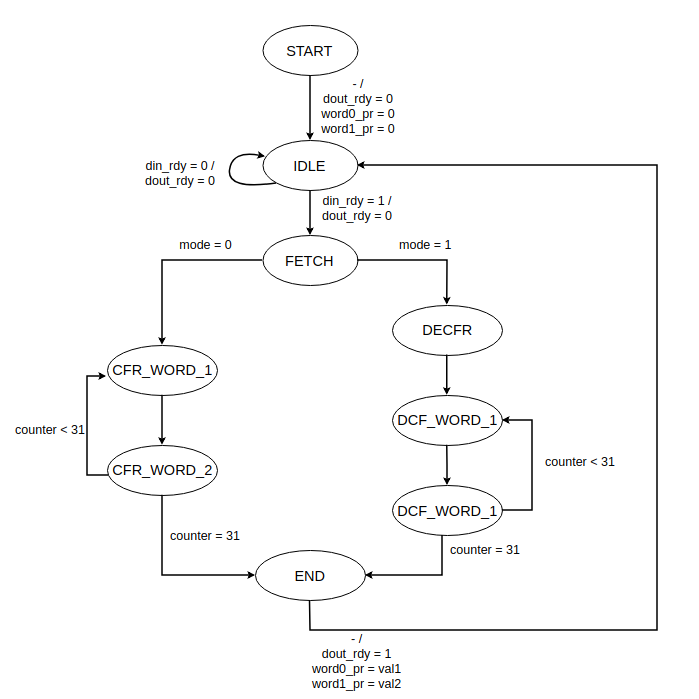
\includegraphics[width=\columnwidth]{Images/scheme6.png}
	\captionof{figure}{EFSM ottenuta partendo dall'algoritmo Xtea. Per ogni arco sono riportati solo i valori significativi per non creare confusione. Si sottolinea inoltre che ogni stato è collegato implicitamente allo stato di reset qualora l'omonimo ingresso venga posto a 1.}
	\label{scheme6}
\end{center}
Una volta realizzata la EFSM, l'implementazione del modulo in systemC non è stata troppo complicata. È stato definito un SC\_MODULE con delle porte di input e output identiche a quelle specificate sopra e con lo stesso tipo dei campi usati a TLM. Inoltre si sono specificati dei segnali interni da usare come delle variabili durante la computazione. Infine sono stati definiti due SC\_METHOD: uno relativo al datapath, sensibile al clock ed a reset, il cui scopo era quello di aggiornare lo stato corrente e, sulla base del nuovo stato, eseguire le operazioni previste o, eventualmente, resettare il modulo; l'altro relativo alla FSM, sensibile al cambiamento sullo stato attuale e  al din\_rdy, con lo scopo di calcolare lo stato prossimo sulla base di stato corrente ed input ricevuti. Durante la realizzazione di questo modulo si è inoltre presa la scelta progettuale di avere un sistema che, fino ad un eventuale reset, continui ad emettere come output il risultato del calcolo precedente piuttosto che un sistema che emetta un output valido solo una volta dopo la computazione e poi lo annulli.

Tutto il modulo è stato poi verificato tramite un testbench ad esso collegato. Si vuole sottolineare inoltre che il ruolo del testbench è stato fondamentale non solo per la verifica del modulo ma anche per la futura implementazione dei transattori e del controllore.


Dopo aver verificato l'effettivo funzionamento del modulo in RT si è poi passati a lavorare sulla parte in AMS sistema, iniziando a progettare la cisterna con una progettazione di tipo LSF.

\subsection{Cisterna LSF}
Essendo la parte riguardante la cisterna dell'acqua e la valvola collegata espresse tramite valori reali ed a tempo continuo si è dovuto progettare questi moduli usando la modellazione AMS fornita da SystemC-ams.

Il primo modulo implementato è stata la cisterna d'acqua. Poiché dalle specifiche fornite si notava che l'evoluzione dell'acqua nella cisterna era data dall'equazione differenziale $ x' = 0,6a-0,03x$, di variabili $x$ e $a$ si è deciso di rappresentare questo modulo usando la rappresentazione LSF, in quanto già fornita delle componenti utili per effettuare i calcoli necessari. Si è quindi proceduto a convertire l'equazione differenziale in un diagramma a blocchi e, successivamente, ad implementare il suddetto diagramma all'interno di un SC\_MODULE appositamente adattato per gestire segnali ams. La figura \ref{scheme7} mostra lo schema del collegamento dei blocchi lsf all'interno del modulo. Si vuole porre nota sul fatto che all'ingresso e all'uscita del sistema vi sono dei convertitori rispettivamente tdf/lsf e lsf/tdf per poter permettere al modulo di dialogare con le altre componenti ams in libertà.
\begin{center}
	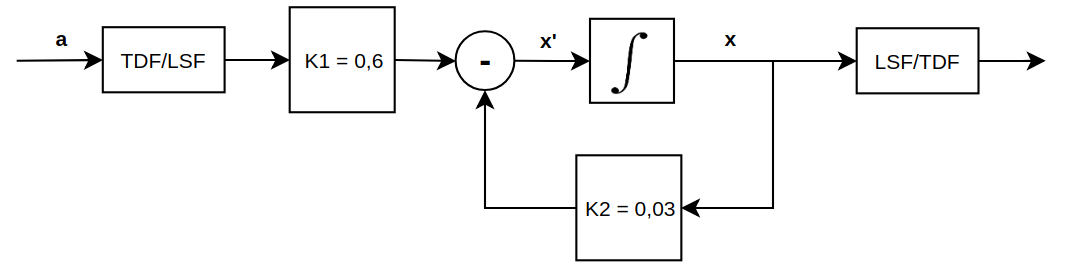
\includegraphics[width=\columnwidth]{Images/scheme7.png}
	\captionof{figure}{Diagramma a blocchi per l'equazione differenziale della cisterna.}
	\label{scheme7}
\end{center}

\subsection{Valvola TDF}
Subito dopo aver implementato la cisterna d'acqua si è passati all'implementazione della valvola. In questo caso però, dato che la valvola deve svolgere anche una funzione di controllo dettata dai comandi inviategli, si è resa necessaria un'implementazione secondo il modello TDF. Per fare ciò si è creato un modulo SCA\_TDF\_MODULE al cui interno sono state definite le porte di ingresso ed uscita (di tipo sca\_tdf::sca\_in e sca\_tdf::sca\_out) ed una variabile interna in cui è salvata l'apertura corrente della valvola. Il modulo presenta inoltre le funzioni \emph{set\_attribute} con la quale è possibile inizializzare i time-step ed i delay delle porte (inizializzate solo in questo modulo e propagate grazie all'upstream e al downstream effettuato da SystemC-ams) ed il metodo \emph{processing}, invocato ad ogni time step. Proprio questo metodo svolge la funzione di controllo, andando a leggere il comando dalla relativa porta e andando a modificare il valore dell'apertura tramite un'operazione di integrazione (in quanto la specifica fa riferimento solamente alla velocità di apertura) data dalla formula: $\text{apertura}=\text{apertura}+0,25\cdot(\text{time step in secondi})$.
\begin{center}
	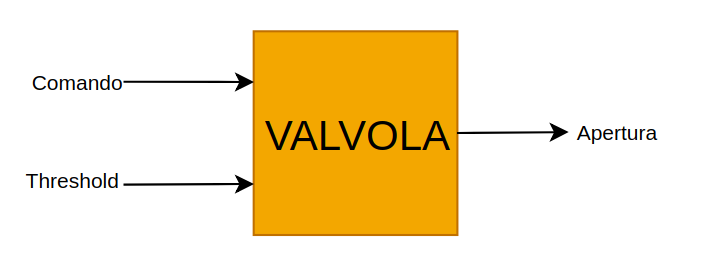
\includegraphics[width=\columnwidth]{Images/scheme8.png}
	\captionof{figure}{Interfaccia della valvola.}
	\label{scheme8}
\end{center}

Dopo aver implementato sia la cisterna che la valvola si è poi passati ad una fase di testing. In un primo momento si è optato per creare un testbench con funzionalità di controllore, il tutto in ams. Successivamente, per incontrare meglio le specifiche del progetto, si è deciso di creare un controllore in TLM LT separato dal testbench. Ovviamente per poter far dialogare il controllore con i moduli ams è stato necessario inserire dei transattori basati parzialmente sul testbench precedente. Uno schema del risultato ottenuto è riportato in figura \ref{scheme9}.

\begin{figure*}[ht]
	\centering
	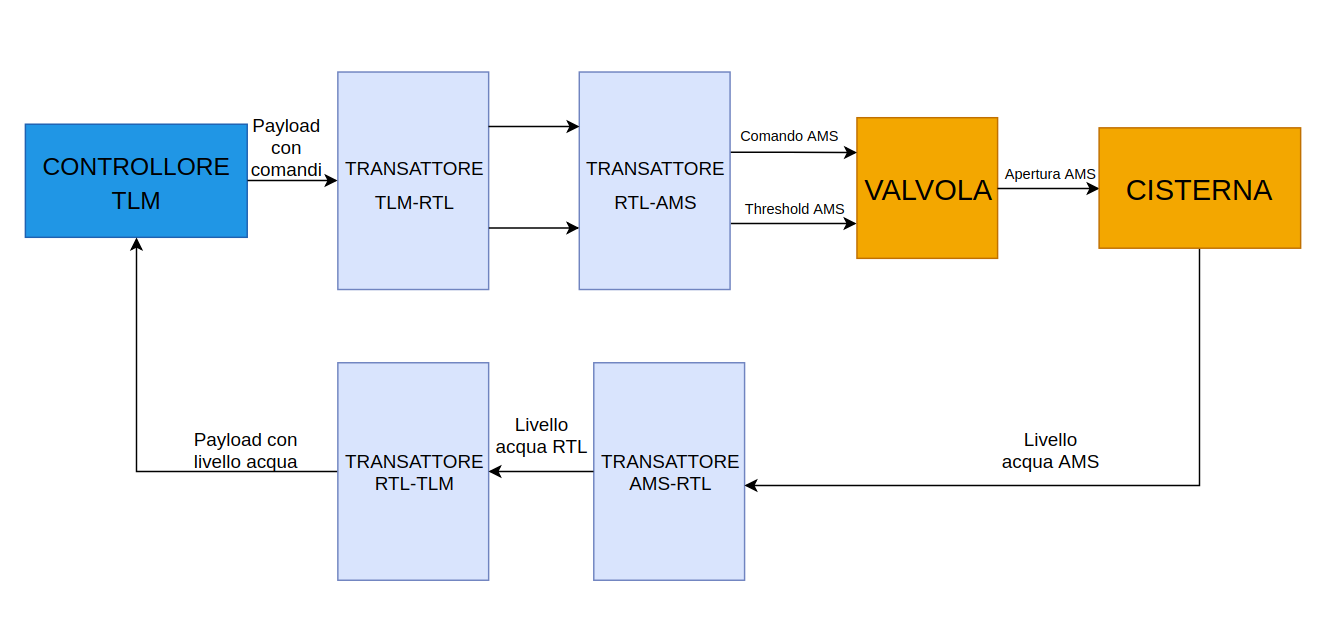
\includegraphics[width=\textwidth]{Images/scheme9.png}
	\caption{Schema del testbench per la parte ams.}
	\label{scheme9}
\end{figure*}

\subsection{Transattori}
Con l'implementazione di un controllore in TLM per la parte AMS si è reso necessario un meccanismo di comunicazione tra i diversi stili di progettazione. Per permettere ciò si sono dovuti implementare diversi transattori, in quanto il dialogo tra AMS e TLM è possibile solo passando attraverso RTL.
Si sono quindi implementati i seguenti transattori:
\begin{itemize}
	\item Transattore TLM-RTL: Modulo SystemC che implementa un'interfaccia TLM LT e che possiede un numero di porte di output pari al numero di campi presenti nel payload. Alla chiamata della funzione \emph{b\_transport} i valori del payload vengono scritti sulle rispettive porte.
	\item Transattore RTL-AMS/AMS-RTL: Modulo SystemC-ams che utilizza le porte sca\_tdf::sca\_de::sca\_in per la conversione automatica da RTL a AMS. Ciò che viene letto su queste porte può essere scritto immediatamente sulle porte di output.
	\item Transattore RTL-TLM: Modulo SystemC con una SC\_THREAD in loop. Per simulare il ritardo della computazione del controllore la thread è impostata per agire ogni cinque secondi di simulazione. Passato tale intervallo la thread invoca la \emph{b\_transport} del controllore inviando un payload con i dati letti dalle porte di input.
\end{itemize}
Bisogna però infine sottolineare che l'aggiunta dei transattori aumenta i tempi di simulazione e produce anche un modifica della curva ottenuta dalla simulazione stessa, in quanto le porte ams di questi ritardano la computazione. Per risolvere ciò è sufficiente abbassare il tempo di attesa del controllore da cinque secondi a quattro (figura \ref{ams}) .
\subsection{Piattaforma eterogenea}
Dopo aver completato la progettazione della parte AMS con controllore, si è infine passati a comporre il sistema finale andando ad unire tutte le componenti precedenti. Osservando la figura \ref{scheme} si può notare come il modulo Xtea sia esattamente a metà strada tra il controllore, definito in TLM, e la valvola, definita in AMS. Grazie a ciò è stato possibile andare a riutilizzare i transattori precedentemente definiti ed in particolare quelli per la conversione da TLM a RTL e da RTL a AMS che sono stati infatti modificati per poter dialogare con il modulo aggiunto. Inoltre è stato necessario apportare alcune modifiche anche al controllore principale.
Più in dettaglio, le modifiche fatte sono state le seguenti:
\begin{itemize}
	\item Modificare il payload dal controllore al transattore in modo che potesse contenere tutte le informazioni utili in futuro al modulo Xtea. Per fare ciò ci si è basati sul payload usato durante la progettazione di Xtea in TLM.
	\item Aggiungere una funzione per la criptazione dei dati al controllore. Per non dover complicare ulteriormente il modulo Xtea (progettato per la cifratura di valori interi) si è deciso di non cifrare il valore della threshold ma solo quello del comando.
	\item Si è modificato il transattore da TLM ad RTL. Questo si è visto complicarsi le proprie funzionalità in quanto ora possiede una SC\_THREAD sensibile a clock (e quindi si è passati ad un modulo sincrono) ed in attesa di un evento invocato solo all'arrivo di un payload (quindi solo all'invocazione della funzione \emph{b\_transport}). Una volta sbloccata, la thread provvede a resettare lo stato del modulo Xtea e solo a questo punto scrivere i dati sulle porte di output.
	\item  Si è modificato il transattore da RTL ad AMS per permettere di accettare le porte di uscita del modulo Xtea (le due parole processate e il dout\_rdy). Il modulo ora ricostruisce la parola originale, spezzata per poter soddisfare gli input della decriptazione, e la emette assieme alla threshold come output. In questo punto si è fatta a scelta progettuale di ignorare il valore della porta dout\_rdy di Xtea poiché, essendo i due moduli progettati per lavorare a frequenze diverse, capitava spesso che il transattore non riuscisse a leggere il valore della porta in tempo prima che questa venisse resettata a 0.
\end{itemize}
Infine per poter procedere alla simulazione è stato allestito un testbench con clock in cui i moduli sono stati collegati e testati. La figura \ref{scheme10} mostra la piattaforma finale.
\begin{figure*}[htb]
	\centering
	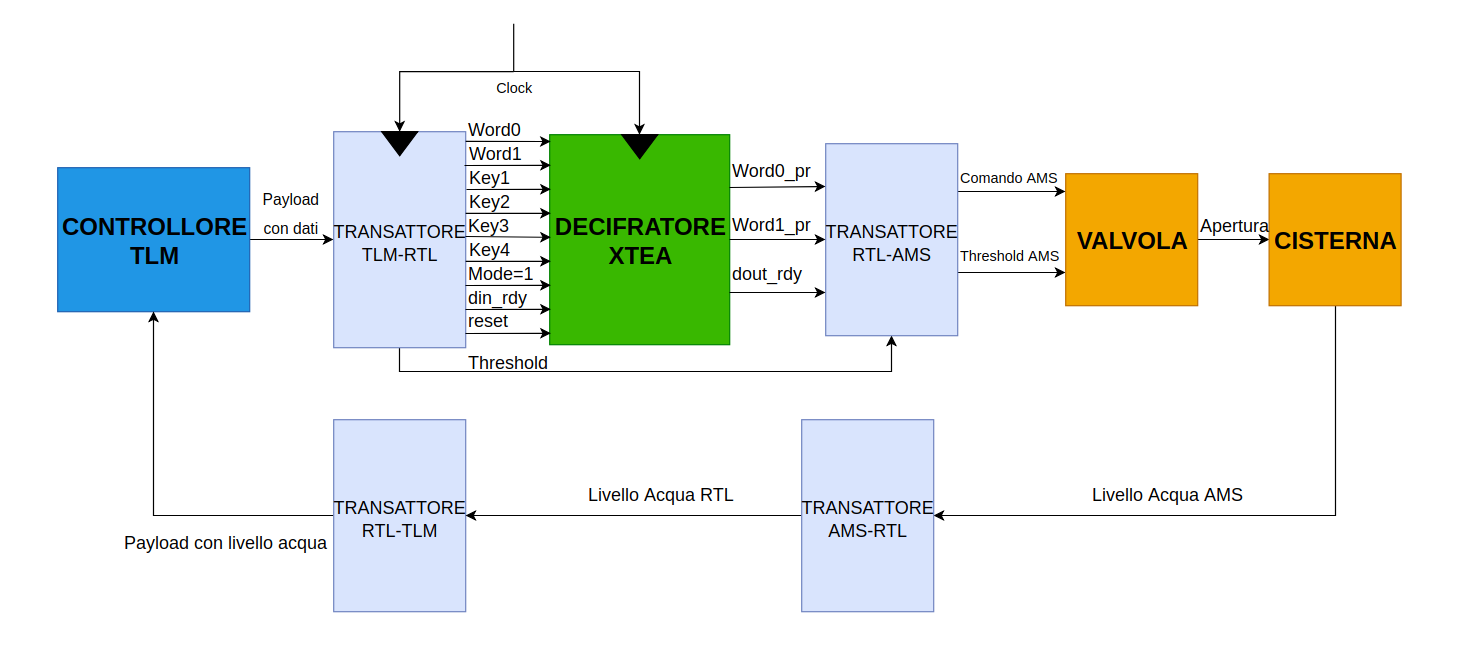
\includegraphics[width=\textwidth]{Images/scheme10.png}
	\caption{Schema dell'impianto finale}
	\label{scheme10}
\end{figure*}

\section{Risultati}
Durante lo sviluppo del sistema, ogni qualvolta una componente fosse stata ultimata, si sono svolte delle fasi di testing per assicurare il corretto funzionamento del modulo completato. Per fare ciò lo si è collegato ad un testbench capace sia di fornire tutti gli input utili alla componente per funzionare, sia di verificare che gli input prodotti rispettassero le specifiche del sistema.

Il primo modulo completato, e quindi soggetto a testing, è stato il modulo Xtea. Essendo stato progettato a diversi livelli di astrazione, prima di ogni raffinamento è stato verificato il suo funzionamento per assicurare che le funzionalità non venissero perse. Analizzando i risultati delle simulazioni ai livelli TLM UT, TLM LT e TLM AT4 si può notare come, oltre ad avere un tempo di esecuzione molto basso, i tempi siano praticamente coincidenti, andando a differenziarsi solo a causa della schedulazione.

 Quanto detto non vale invece per la simulazione a livello RT. In primo luogo questa risulta più lenta delle precedenti ma la vera differenza è data dal fatto che SystemC, per la simulazione RTL, permette di tracciare l'evoluzione dei segnali secondo il tempo di simulazione e, di conseguenza, anche il tempo che effettivamente verrebbe impiegato dal sistema nella realtà. Un esempio di ciò è dato dalla figura \ref{wave1} che, in sintesi, mostra che il modulo impiega circa 680 ns per completare un intero ciclo di criptazione o decriptazione partendo dallo stato di reset (con un periodo di clock pari a 10 ns).

\begin{figure*}[htb]
	\centering
	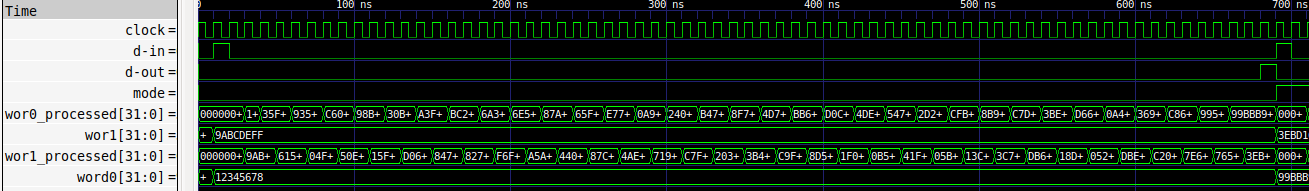
\includegraphics[width=\textwidth]{Images/wave1.png}
	\caption{Traccia dei segnali principali del modulo Xtea a RTL. Si noti che al tempo 680 ns il valore del dout\_rdy viene alzato per informare il testbench che la computazione è terminata. Al ciclo di clock successivo il testbench risponde a ciò con una nuova computazione, in decifratura (da notare la modalità) ed alzando il din\_rdy.}
	\label{wave1}
\end{figure*}
Successivamente si è testato la parte in AMS. Inizialmente si sono eseguiti dei test con un sistema AMS puro per verificare che il valore dell'acqua nella cisterna si stabilizzi. Ottenuto tale risultato è stato inserito il controller TLM con i relativi transattori e si è proceduto con ulteriori test. Come è possibile vedere dalla figura \ref{ams} il valore dell'acqua si stabilizza ma sono presenti due picchi. Ciò è dovuto al ritardo nella computazione che i transattori creano ed è rimediabile abbassando la frequenza di controllo del controllore da cinque a quattro secondi senza che ciò impatti i tempi di simulazione % che resta fissa attorno ai 20 secondi 
e il tempo per la stabilizzazione, fisso a 300 secondi
Facendo ciò però si cambia anche il valore che il livello d'acqua assume a regime, passando da 6,25 a 8,5 (sempre figura \ref{ams}).

\begin{figure*}[htb]
	\centering
	\minipage{0.47\textwidth}
	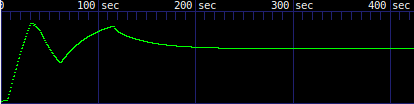
\includegraphics[width=\columnwidth]{Images/AMS-5sec.png}
	\endminipage\hfill
	\minipage{0.51\textwidth}
	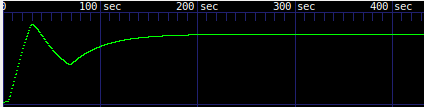
\includegraphics[width=\columnwidth]{Images/AMS-4sec.png}
	\endminipage\hfill
	\centering

	\caption{Simulazione del sistema AMS con transattori e tempo di reazione del controllore a cinque (sinistra) e quattro (destra) secondi .}
	\label{ams}
\end{figure*}
Infine è stato testato il sistema finale con la stesa metodologia sopra riportata. In questo caso, tuttavia, si è reso necessario alzare la frequenza del clock passando dai nanosecondi ai microsecondi. Le differenze di tempistiche dei moduli, infatti rallenta incredibilmente la simulazione e, poiché per rispettare il comportamento del sistema basta che il modulo Xtea (unico beneficiario del clock) sia più veloce degli altri moduli, si è deciso di abbassare il rapporto tra velocità del clock e time step delle porte AMS da $10^6$ a $10^3$ andando ad ottenere una simulazione con tempistiche accettabili e al contempo mantenendo la correttezza dell'architettura, come mostrano i risultati ottenuti, praticamente identici a quelli trovati testando la versione in AMS. Anche in questo caso abbassando la frequenza di controllo da cinque a quattro secondi si può notare come il secondo picco sparisca (figura \ref{het}).
\begin{figure*}[htb]
	\centering
	\minipage{0.47\textwidth}
	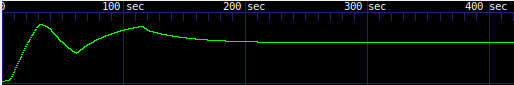
\includegraphics[width=\columnwidth]{Images/heterogeneus_5sec.png}
	\endminipage\hfill
	\minipage{0.51\textwidth}
	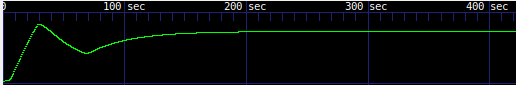
\includegraphics[width=\columnwidth]{Images/heterogeneus_4sec.png}
	\endminipage\hfill
	\centering

	\caption{Simulazione del sistema finale con tempo di reazione del controllore a cinque (sinistra) e quattro (destra) secondi .}
	\label{het}
\end{figure*}
\section{Conclusioni}
Osservando quanto fatto nel corso del progetto ed i risultati ottenuti ci si rende subito conto di un fatto molto importante: quanto ottenuto non si sarebbe potuto ottenere nei tempi e modi in cui si è fatto se non vi fossero stati presenti due elementi chiave. Primo di questi è una metodologia di sviluppo in grado di permettere la creazione di componenti funzionanti e corrette tramite una serie di raffinamenti, riusi di parti precedentemente verificate e test per ridurre al minimo la riscrittura di codice e aumentare quindi la velocità di produzione. Secondo elemento fondamentale è stato il supporto che SystemC ha fornito. Poter definire componenti utilizzando classi o  moduli già implementati dalla libreria stessa, collegare tra loro queste componenti in un modo facile e quasi intuitivo avendo la possibilità di testare i moduli hardware digitali o analogici e, allo stesso tempo, poter osservare il loro comportamento senza dover realizzare l'hardware stesso, fanno la differenza per poter creare un hardware già funzionante e affidabile, limitando di molto il rischio di dover ri-sintetizzare tutto di nuovo sprecando tempo e risorse. Questo progetto ha messo quindi in evidenza che la combinazione di questi due fattori permette lo sviluppo di un sistema funzionante nonostante la non banalità di quest'ultimo, in tempi abbastanza brevi e con dei risultati soddisfacenti.


\bibliographystyle{IEEEtran}
\bibliography{biblio}

\end{document}